\documentclass{sigchi}

% Use this command to override the default ACM copyright statement (e.g. for preprints). 
% Consult the conference website for the camera-ready copyright statement.
\toappear{
	Submitted for review.
}

% Arabic page numbers for submission. 
% Remove this line to eliminate page numbers for the camera ready copy
\pagenumbering{arabic}


% Load basic packages
\usepackage{balance}  % to better equalize the last page
\usepackage{graphics} % for EPS, load graphicx instead
\usepackage{times}    % comment if you want LaTeX's default font
\usepackage{url}      % llt: nicely formatted URLs

% llt: Define a global style for URLs, rather that the default one
\makeatletter
\def\url@leostyle{%
  \@ifundefined{selectfont}{\def\UrlFont{\sf}}{\def\UrlFont{\small\bf\ttfamily}}}
\makeatother
\urlstyle{leo}


% To make various LaTeX processors do the right thing with page size.
\def\pprw{8.5in}
\def\pprh{11in}
\special{papersize=\pprw,\pprh}
\setlength{\paperwidth}{\pprw}
\setlength{\paperheight}{\pprh}
\setlength{\pdfpagewidth}{\pprw}
\setlength{\pdfpageheight}{\pprh}

% Make sure hyperref comes last of your loaded packages, 
% to give it a fighting chance of not being over-written, 
% since its job is to redefine many LaTeX commands.
\usepackage{hyperref}
\hypersetup{
pdftitle={NFC Authorized Outlet},
pdfauthor={LaTeX},
pdfkeywords={SIGCHI, proceedings, archival format},
bookmarksnumbered,
pdfstartview={FitH},
colorlinks,
citecolor=black,
filecolor=black,
linkcolor=black,
urlcolor=black,
breaklinks=true,
}

% create a shortcut to typeset table headings
\newcommand\tabhead[1]{\small\textbf{#1}}


% End of preamble. Here it comes the document.
\begin{document}

\title{NFC Authorized Outlet}

\numberofauthors{3}
\author{
  \alignauthor Ryan Fahsel\\
    \affaddr Georgia Institute of Technology\\
%    \affaddr{Address}\\
    \email ryan.fahsel@gatech.edu\\
%    \affaddr{Optional phone number}
  \alignauthor Colin Gray\\
    \affaddr Georgia Institute of Technology\\
%    \affaddr{Address}\\
    \email colin.gray@gatech.edu\\
%    \affaddr{Optional phone number}    
  \alignauthor Ramya Ramakrishnan\\
    \affaddr Georgia Institute of Technology\\
%    \affaddr{Address}\\
    \email rramakrishnan3@gatech.edu\\
%    \affaddr{Optional phone number}
}

\maketitle

\begin{abstract}
In this project, an authorization system was implemented using the NFC technology on mobile devices. The motivation behind this research was to make authorization of tools in a lab easier and more effective. This way, users would be allowed to enter labs but restricted to use certain tools. Previous studies have looked into RFID and NFC technologies for many applications, such as for hospitals and virtual ticketing systems. In our work, we have implemented a system that controls a 120 volt outlet which will provide or restrict access to the user based on their credentials. We use the mobile device as an NFC reader and attach NFC stickers to each tool that act as tags. We implemented the hardware and software sides and a site that allows us to manage the user permissions. From this project, we learned that the NFC technology embedded in our phones is an effective way to transmit the credentials of users. In future work, we hope to...
\end{abstract}

\keywords{
	NFC; RFID; Authorization.
%	\textcolor{red}{Mandatory section to be included in your final version.}
}

\category{H.5.m.}{}{}


\terms{
	Human Factors; Security. 
}

%See list of the limited ACM 16 terms in the
%instructions and additional information:
%\url{http://www.sheridanprinting.com/sigchi/generalterms.htm}.
%\textcolor{red}{Optional section to be included in your final version.}

\section{Introduction}

\subsection {Project Description}
The goal of this project was to create an access controlled, household 120v outlet. The system is composed of an Android application, web server backend, and Adurino controlled circuit. The best way to describe how the system works is through the following example: Alice wants to use the prototyping lab. She attends the mandatory training session and is given access to the lab. This is great for tools like the screwdrivers, hammers, and other small tools; however, how can the lab owners control access to potentially dangerous tools (i.e. saws, waterjets, etc)? This is how. A user comes up to a saw, opens an Android application, and taps his or her phone against an NFC tag on the desired tool. The phone sends a request to a webserver with the user’s credentials. The web server checks a database to see if the requestor is authorized to use the desired tool; if he or she is, the outlet the tool is connected to is powered; if he or she is not, the outlet to the tool remains powered off. While all of this sounds complicated, it happens in less than five seconds. The outlet is ‘powered’ or ‘not powered’ by a relay, which is controlled by an Adurino board. Additionally, there will be a locking mechanism that prohibits a user from unplugging a device and plugging it into another outlet that is not access controlled.

\subsection {Motivation}

The idea of access control to locked areas via RFID is not a new idea; however, using NFC to control outlets is though. When Scott Gullivan came to give a presentation on project ideas; he expressed the desire to be able to grant access to the lab to a large set of people, while only allowing a subset of ‘trained’ users to use some of the more dangerous tools; however, Scott did not want to go purchase all new tools that had authentication built into them. Even if Scott was starting a new lab from scratch, he would not want to go and limit himself to only tools that have authentication built into them (which as far we know, do not even exist). There has to be a way to access control tools that already exist in the lab; the only way to do that is to control the power given to the tools. This creates a cheap and universal way (via a standard 120v plug) to grant a large group of people access to a space, while only allowing a subset of those people to use the devices within a space. 

NFC is the technology of choice for this control because it is way more robust than RFID. NFC tags can store much more data than RFID and NFC readers are becoming commonplace in phones, which is an object a majority of people carry around with them daily.

This research is based on figuring out if this is ‘doable’. Once this is discovered, this technology can be scaled to much larger uses. For example, airports could build this technology into all their outlets; thus, people have to be authorized (essentially pay) to use the outlets, which is much more convenient than charging stations that require a user to awkwardly stand in the middle of a terminal for long periods of time. 

\section{Previous/Related Work}

Several past studies have analyzed the benefits of NFC and RFID technologies for authentication and have implemented systems using these for applications such as healthcare monitoring, ticketing systems, etc. One study looked at NFC capabilities for mobile interactions and concluded that NFC in mobile phones can be used for ticketing, mobile payment, and authentication. This was determined through field trials and through analysis of current use of NFC. Some of the current systems using NFC include accessing public transportation in the Paris Metro System and managing stock in the Finnish company JCDecaux Finland Oy (Falke et al. 8). In this research, we hope to explore the idea of using NFC for controlling access to lab equipment, and since more phones are starting to be equipped with NFC, there can be more potential for work in this area. We hope to use the useful NFC technology embedded in phones to make access control as simple as possible.

Another study looked at using NFC for health care systems to facilitate more efficient patient treatment. Because staff members often have to treat a large number of patients, there is a chance that the wrong medication will be given to a patient. In order to avoid this type of error, NFC technologies can be used to ensure that the correct medication is given to each patient (Lahtela 242). NFC has been further studied for other applications such as virtual ticketing. An application called NFCTicketing was created to allow users to buy public transportation tickets using their phone (Ghiron 46). 

Haselsteiner also described the capability of NFC technologies to be used in ticketing and micropayment. In his explanation, he details how contactless Smart Cards or phones with embedded NFC technology can be used to communicate with a reader, which can accept or reject the ticket (3). Similarly, we want to create a simple system that allows a reader to receive information from a phone and accept or reject access to the piece of lab equipment, based on the user’s credentials. 

Overall, many of these past studies have studied the use of NFC in hospitals and virtual ticketing systems and have outlined the potential of using NFC technologies. We would like to extend this use of NFC by implementing a system to control access to lab equipment by enabling and disabling a 120 volt outlet with phones as our NFC reader and NFC stickers as our tags.

\section{Our Work}

\subsection {Resources}
There are three main components to this project: an NFC enabled Android device, a webserver, and an Adurino controlled circuit. Additionally, we need an aesthetically pleasing and easy to use housing for the circuit.
\begin{itemize}
\item NFC enabled Android device: We own a Nexus 7 which is NFC enabled.
\item Webserver: Georgia Tech offers free hosting to all students. We plan on using this to run a Fedora powered webserver with PHP and MySQL access.
\item Adurino powered circuit: Adurinos and basic relays are relatively cheap. Our group has agreed that the costs associated with buying these materials is less than \$100 total, which we are willing to absorb.
\item Housing: We will use the tools in the protoying lab to create a box (most likely of acryllic, which is easily obtainable from Home Depot).
\end{itemize}
We believe we have all of our resources taken care of and are ready to begin this project.

\subsection{Implementation}
In order to implement this project, we first completed the database design, in which we included tables for storing the users of the application, the tools that our system would include, and the permissions specifying which users had access to those tools. 
We established a connection to the server via our Android device.
We programmed NFC tags and implemented the NFC component of the Android app.
To make changes to the database, we made a site that had the functionality of adding/deleting users and managing the permissions that these users had for the tools in our database.
On the hardware side, we created a circuit..... and designed a housing for this circuit.

\subsection {Functionality}
The deliverable of this project was a system that allowed outlets to be turned on by authorized users by tapping their Android phone against an NFC tag associated with an outlet. The following enumerates the basic functionality of this system:
\begin{itemize}
\item The application can read NFC tags and send them to the web server.

\item The system can distinguish between authorized and unauthorized users trying to power outlets and make decisions accordingly. 

\item The controllable outlets should be protected in such a way that users (with the exception of authorized administrators) cannot remove the plugs of devices from the controlled outlet to plug into another outlet.
\end{itemize}

\section{Discussion}

The results of this project had several important findings. One was that using the NFC technology built into the Android device was an effective way to transmit information about the user. This was easily used to determine whether the user was authorized to use the tool. The NFC stickers were simple to use and worked well with the NFC embedded in our mobile device. We had no issues with the transmission of information between the sticker and our phone. So, this system could be implemented in a larger scale because phones with embedded NFC are much more common and NFC stickers can be easily incorporated.

Another finding was that the time taken for the tool to turn on after tapping the device next to the NFC tag was slightly longer than we expected. We don't, however, see much potential for improvement here because of the time taken to transmit information to the server.

Although this technology worked well for the tools that we tested, we realize that in order for our system to work effectively, we would have to associate an NFC tag with every tool that we want to incorporate. Thus, there are difficulties in implementing this in the real world. However, we feel that the benefit of this system is higher than the cost of setting up NFC tags for each tool.

\section{Future Work}


\section{Conclusion}


%\begin{figure}[!h]
%\centering
%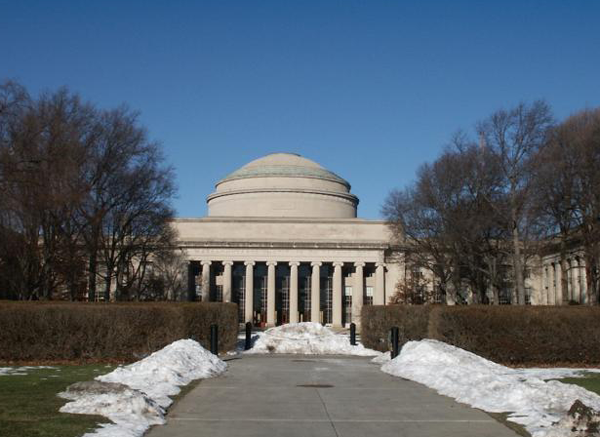
\includegraphics[width=0.9\columnwidth]{Figure1}
%\caption{With Caption Below, be sure to have a good resolution image
%  (see item D within the preparation instructions).}
%\label{fig:figure1}
%\end{figure}

\section{References}

\begin{enumerate}
\item Falke, Oliver, et al. "Mobile services for near field communication." University of Munich, Department of Computer Science, Media Informatics Group, Tech. Rep., LMU-MI-2007-1 (2007).

\item Ghiron, S.L.; Sposato, S.; Medaglia, C.M.; Moroni, A.; "NFC Ticketing: A Prototype and Usability Test of an NFC-Based Virtual Ticketing Application," Near Field Communication, 2009. NFC '09. First International Workshop on , vol., no., pp.45-50, 24-24 Feb. 2009.

\item Haselsteiner, Ernst, and Klemens Breitfuß. "Security in near field communication (NFC)." Workshop on RFID Security RFIDSec. 2006.

\item Lahtela, A.; Hassinen, M.; Jylha, V.; , "RFID and NFC in healthcare: Safety of hospitals medication care," Pervasive Computing Technologies for Healthcare, 2008. PervasiveHealth 2008. Second International Conference on , vol., no., pp.241-244, Jan. 30 2008-Feb. 1 2008.
\end{enumerate}

%\begin{table}
%  \centering
%  \begin{tabular}{|c|c|c|}
%    \hline
%    \tabhead{Objects} &
%    \multicolumn{1}{|p{0.3\columnwidth}|}{\centering\tabhead{Caption --- pre-2002}} &
%    \multicolumn{1}{|p{0.4\columnwidth}|}{\centering\tabhead{Caption --- 2003 and afterwards}} \\
%    \hline
%    Tables & Above & Below \\
%    \hline
%    Figures & Below & Below \\
%    \hline
%  \end{tabular}
%  \caption{Table captions should be placed below the table.}
%  \label{tab:table1}
%\end{table}


\section{Acknowledgments}

We thank Dr. Gregory D. Abowd, Dr. Thad Starner, Clint Zeagler, and Caleb Southern for leading the class Mobile and Ubiquitous Computing, which was the inspiration for this project.

% Balancing columns in a ref list is a bit of a pain because you
% either use a hack like flushend or balance, or manually insert
% a column break.  http://www.tex.ac.uk/cgi-bin/texfaq2html?label=balance
% multicols doesn't work because we're already in two-column mode,
% and flushend isn't awesome, so I choose balance.  See this
% for more info: http://cs.brown.edu/system/software/latex/doc/balance.pdf
%
% Note that in a perfect world balance wants to be in the first
% column of the last page.
%
% If balance doesn't work for you, you can remove that and
% hard-code a column break into the bbl file right before you
% submit:
%
% http://stackoverflow.com/questions/2149854/how-to-manually-equalize-columns-
% in-an-ieee-paper-if-using-bibtex
%
% Or, just remove \balance and give up on balancing the last page.
%
\balance

% If you want to use smaller typesetting for the reference list,
% uncomment the following line:
% \small
%\bibliographystyle{acm-sigchi}
%\bibliography{sample}
\end{document}
